\documentclass[14pt, a4paper]{article}

\usepackage{ucs}
\usepackage{amssymb}
\usepackage{extsizes}
\usepackage{graphicx}
\usepackage{xcolor}
\usepackage{caption}
\usepackage{listings}
\usepackage{tabularx}
\usepackage{indentfirst}
\usepackage[T2A]{fontenc}
\usepackage[utf8]{inputenc}
\usepackage[english,russian]{babel}
\usepackage[left=30mm, right=10mm, top=20mm, bottom=20mm]{geometry}

\graphicspath{{images/}}

\linespread{1.3}
\setcounter{tocdepth}{4}
\setlength{\parskip}{1.5pt}

\lstdefinestyle{asm}{
	language={[x86masm]Assembler},
	backgroundcolor=\color{white},
	basicstyle=\footnotesize\ttfamily,
	keywordstyle=\color{blue},
	stringstyle=\color{red},
	commentstyle=\color{gray},
	numbers=left,
	numberstyle=\tiny,
	stepnumber=1,
	numbersep=5pt,
	frame=single,
	tabsize=4,
	captionpos=b,
	breaklines=true
}

\lstset{basicstyle=\fontsize{10}{10}\selectfont,breaklines=true,inputencoding=utf8x,extendedchars=\true}

\lstset{
	literate=
	{а}{{\selectfont\char224}}1
	{б}{{\selectfont\char225}}1
	{в}{{\selectfont\char226}}1
	{г}{{\selectfont\char227}}1
	{д}{{\selectfont\char228}}1
	{е}{{\selectfont\char229}}1
	{ё}{{\"e}}1
	{ж}{{\selectfont\char230}}1
	{з}{{\selectfont\char231}}1
	{и}{{\selectfont\char232}}1
	{й}{{\selectfont\char233}}1
	{к}{{\selectfont\char234}}1
	{л}{{\selectfont\char235}}1
	{м}{{\selectfont\char236}}1
	{н}{{\selectfont\char237}}1
	{о}{{\selectfont\char238}}1
	{п}{{\selectfont\char239}}1
	{р}{{\selectfont\char240}}1
	{с}{{\selectfont\char241}}1
	{т}{{\selectfont\char242}}1
	{у}{{\selectfont\char243}}1
	{ф}{{\selectfont\char244}}1
	{х}{{\selectfont\char245}}1
	{ц}{{\selectfont\char246}}1
	{ч}{{\selectfont\char247}}1
	{ш}{{\selectfont\char248}}1
	{щ}{{\selectfont\char249}}1
	{ъ}{{\selectfont\char250}}1
	{ы}{{\selectfont\char251}}1
	{ь}{{\selectfont\char252}}1
	{э}{{\selectfont\char253}}1
	{ю}{{\selectfont\char254}}1
	{я}{{\selectfont\char255}}1
	{А}{{\selectfont\char192}}1
	{Б}{{\selectfont\char193}}1
	{В}{{\selectfont\char194}}1
	{Г}{{\selectfont\char195}}1
	{Д}{{\selectfont\char196}}1
	{Е}{{\selectfont\char197}}1
	{Ё}{{\"E}}1
	{Ж}{{\selectfont\char198}}1
	{З}{{\selectfont\char199}}1
	{И}{{\selectfont\char200}}1
	{Й}{{\selectfont\char201}}1
	{К}{{\selectfont\char202}}1
	{Л}{{\selectfont\char203}}1
	{М}{{\selectfont\char204}}1
	{Н}{{\selectfont\char205}}1
	{О}{{\selectfont\char206}}1
	{П}{{\selectfont\char207}}1
	{Р}{{\selectfont\char208}}1
	{С}{{\selectfont\char209}}1
	{Т}{{\selectfont\char210}}1
	{У}{{\selectfont\char211}}1
	{Ф}{{\selectfont\char212}}1
	{Х}{{\selectfont\char213}}1
	{Ц}{{\selectfont\char214}}1
	{Ч}{{\selectfont\char215}}1
	{Ш}{{\selectfont\char216}}1
	{Щ}{{\selectfont\char217}}1
	{Ъ}{{\selectfont\char218}}1
	{Ы}{{\selectfont\char219}}1
	{Ь}{{\selectfont\char220}}1
	{Э}{{\selectfont\char221}}1
	{Ю}{{\selectfont\char222}}1
	{Я}{{\selectfont\char223}}1
}

\begin{document}
	\thispagestyle{empty}
	
	\noindent
	\begin{minipage}{0.15\linewidth}
		
\includegraphics[width=\linewidth]{b_logo}
	\end{minipage}
	\begin{minipage}{0.85\linewidth}\centering
		\footnotesize
		\bf{Министерство науки и высшего образования Российской Федерации}\\
		\bf{Федеральное государственное бюджетное образовательное учреждение высшего образования}\\
		\bf{«Московский государственный технический университет имени Н.Э.~Баумана}\\
		\bf{(национальный исследовательский университет)»}\\
		\bf{(МГТУ им. Н.Э.~Баумана)}
	\end{minipage}
	\newline
	\newline
	\noindent\rule{\textwidth}{3pt}

	\noindent
 	\small ФАКУЛЬТЕТ {\bf <<ИНФОРМАТИКА И СИСТЕМЫ УПРАВЛЕНИЯ>>}\\
	
	\noindent
	\small КАФЕДРА {\bf<<ПРОГРАММНОЕ ОБЕСПЕЧЕНЕ ЭВМ И ИНФОРМАЦИОННЫЕ ТЕХНОЛОГИИ>>}\\
	
	\noindent
	\small НАПРАВЛЕНИЕ ПОДГОТОВКИ {\bf 09.03.04 <<ПРОГРАММНАЯ ИНЖЕНЕРИЯ>>}\\
	
	\vspace{3cm}

	\noindent
	\begin{minipage}{\linewidth}
		\centering\large\bf{ОТЧЕТ}

		\centering\bf{по лабораторной работе №1}
	\end{minipage}
	
	\vspace{2cm}
	
	\noindent {\bf Название:} \underline{Дизассемблирование INT 8h}
	
	\bigbreak
	
	\noindent {\bf Дисциплина:} \underline{Операционные системы}
	
	\vspace{2cm}
	
	\noindent
	\begin{center}
		\begin{tabularx}{\linewidth}{XXXX}
			\bf Студент &&& \underline{Царев А.А.}\\
			&&&\\
			\bf Группа &&& \underline{ИУ7-53Б}\\
			&&&\\
			\bf Преподаватель &&& \underline{Рязанова Н.Ю.}\\
		\end{tabularx}
	
		\vfill
		
		Москва, \the\year
	\end{center}
	
	\pagebreak
		
	\section*{Введение}
	
	\subsection*{Цель работы}
	
	Знакомство со средством дизассемблирования – sourcer и с получением дизассемблерного кода ядра операционной системы Windows на примере обработчика прерывания Int 8h в virtual mode – специальном режиме защищенного режима, который эмулирует реальный режим работы вычислительной системы на базе процессоров Intel.
	
	\subsection*{Задание}
	
	Используя sourser (sr.exe) получить дизассемблерный код обработчика аппаратного прерывания от системного таймера Int 8h.
	На основе полученного кода составить алгоритм работы обработчика Int 8h.
	
	По данной лабораторной работе составляется отчет в письменном виде.
	
	\pagebreak
	
	\section*{Полученный дизассемблерный код}
	
	\subsection*{Листинг INT 8h}
	
	\begin{lstlisting}[style={asm}]
		; Вызов процедуры sub_2
		020A:0746  E8 0070				call	sub_2			; (07B9)
		
		; Сохранение регистров ES, DS, AX и DX
		020A:0749  06					push	es
		020A:074A  1E					push	ds
		020A:074B  50					push	ax
		020A:074C  52					push	dx
		
		; Запись 0040h в регистр DS
		020A:074D  B8 0040				mov	ax,40h
		020A:0750  8E D8				mov	ds,ax
		
		; Обнуление регистров AX и ES
		020A:0752  33 C0				xor	ax,ax			; Zero register
		020A:0754  8E C0				mov	es,ax
		
		; Инкремент младших двух байт счетчика реального времени
		020A:0756  FF 06 006C				inc	word ptr ds:[6Ch]	; (0040:006C=124Dh)
		020A:075A  75 04				jnz	loc_16			; Jump if not zero
		
		; Инкремент старших двух байт счетчика реального времени
		020A:075C  FF 06 006E				inc	word ptr ds:[6Eh]	; (0040:006E=3)
		
		; Проверка на то, что прошло 24 часа
		; 24 * 60 * 60 * (1193180 / 65536) ~= 1573040 = 1800B0h
		020A:0760			loc_16:
		020A:0760  83 3E 006E 18			cmp	word ptr ds:[6Eh],18h	; (0040:006E=3)
		020A:0765  75 15				jne	loc_17			; Jump if not equal
		020A:0767  81 3E 006C 00B0			cmp	word ptr ds:[6Ch],0B0h	; (0040:006C=124Dh)
		020A:076D  75 0D				jne	loc_17			; Jump if not equal
		
		; Если прошло 24 часа, то счетчик реального времени обнуляется, и устанавливается единица по адресу 0040:0070
		020A:076F  A3 006E				mov	word ptr ds:[6Eh],ax	; (0040:006E=3)
		020A:0772  A3 006C				mov	word ptr ds:[6Ch],ax	; (0040:006C=124Dh)
		020A:0775  C6 06 0070 01			mov	byte ptr ds:[70h],1	; (0040:0070=0)
		
		; Запись значения 8 в AL
		020A:077A  0C 08				or	al,8
		
		020A:077C			loc_17:
		
		; Сохранение регистра AX в стеке
		020A:077C  50					push	ax
		
		; Декремент счетчика времени до выключения моторчика
		020A:077D  FE 0E 0040				dec	byte ptr ds:[40h]	; (0040:0040=43h)
		020A:0781  75 0B				jnz	loc_18			; Jump if not zero
		
		; Если счетчик времени до выключения моторчика равен 0, устанавливаем флаги, отвечающие за отключение моторчика
		020A:0783  80 26 003F F0			and	byte ptr ds:[3Fh],0F0h	; (0040:003F=0)
		
		; Отключение моторчика дисковода
		020A:0788  B0 0C				mov	al,0Ch
		020A:078A  BA 03F2				mov	dx,3F2h
		020A:078D  EE					out	dx,al			; port 3F2h, dsk0 contrl output
		
		020A:078E			loc_18:
		
		; Восстановление регистра AX
		020A:078E  58					pop	ax
		
		; Проверяем флаг четности PF
		020A:078F  F7 06 0314 0004			test	word ptr ds:[314h],4	; (0040:0314=3200h)
		020A:0795  75 0C				jnz	loc_19			; Jump if not zero
		
		; Запись младшего байта регистра флагов в AH
		020A:0797  9F					lahf				; Load ah from flags
		020A:0798  86 E0				xchg	ah,al
		
		; Сохранение регистра AX
		020A:079A  50					push	ax
		
		; Косвенный вызов прерывания 1Ch.
		; Вызов осуществляется через call, чтобы при выполнении команды iret
		; в регистр флагов был записан регистр AX, который
		; был сохранен до вызова прерывания
		020A:079B  26: FF 1E 0070			call	dword ptr es:[70h]	; (0000:0070=6ADh)
		020A:07A0  EB 03				jmp	short loc_20		; (07A5)
		020A:07A2  90					nop
		
		020A:07A3			loc_19:
		020A:07A3  CD 1C				int	1Ch			; Timer break (call each 18.2ms)
		
		020A:07A5			loc_20:
		020A:07A5  E8 0011				call	sub_2			; (07B9)
		
		; Сброс контроллера прерываний
		020A:07A8  B0 20				mov	al,20h			; ' '
		020A:07AA  E6 20				out	20h,al			; port 20h, 8259-1 int command
		;  al = 20h, end of interrupt
		
		; Восстановление регистров DX, AX, DS и ES
		020A:07AC  5A					pop	dx
		020A:07AD  58					pop	ax
		020A:07AE  1F					pop	ds
		020A:07AF  07					pop	es
		
		020A:07B0  E9 FE99				jmp	loc_1			; (064C)
		
		; ...
		
		020A:064C			loc_1:
		020A:064C  1E					push	ds
		020A:064D  50					push	ax
		
		; ...
		
		020A:06AA  58					pop	ax
		020A:06AB  1F					pop	ds
		
		020A:06AC  CF					iret				; Interrupt return
	\end{lstlisting}
	
	\subsection*{Листинг процедуры sub\_2}
	
	\begin{lstlisting}[style={asm}]
						sub_2		proc	near
		
		; Сохранение регистров DS и AX
		020A:07B9  1E					push	ds
		020A:07BA  50					push	ax
		
		; Запись 0040h в регистр DS
		020A:07BB  B8 0040				mov	ax,40h
		020A:07BE  8E D8				mov	ds,ax
		
		; Запись младшего байта регистра флагов в AH
		020A:07C0  9F					lahf				; Load ah from flags
		
		; Проверка флага DF и старшего бита флага IOPL
		020A:07C1  F7 06 0314 2400			test	word ptr ds:[314h],2400h	; (0040:0314=3200h)
		020A:07C7  75 0C				jnz	loc_22			; Jump if not zero
		
		; Сброс флага IF в области данных BIOS (в 0040:0314)
		; Команда lock используется для того, чтобы следующая за ней команда
		; была неделимой
		020A:07C9  F0> 81 26 0314 FDFF	           lock	and	word ptr ds:[314h],0FDFFh	; (0040:0314=3200h)
		
		020A:07D0			loc_21:
		
		; Запись регистра AH в младший байт регистра флагов
		020A:07D0  9E					sahf				; Store ah into flags
		
		; Восстановление регистров AX и DS
		020A:07D1  58					pop	ax
		020A:07D2  1F					pop	ds
		020A:07D3  EB 03				jmp	short loc_23		; (07D8)
		
		020A:07D5			loc_22:
		
		; Если установлен хотя бы DF или старший бит IOPL, то происходит сброс флага IF
		020A:07D5  FA					cli				; Disable interrupts
		020A:07D6  EB F8				jmp	short loc_21		; (07D0)
		020A:07D8			loc_23:
		
		; Возврат из процедуры
		020A:07D8  C3					retn
		sub_2		endp
	\end{lstlisting}
	
	\pagebreak
	
	\section*{Схемы алгоритмов}
	
	\subsection*{Схема алгоритма INT 8h}
	
	\begin{minipage}{0.9\linewidth}
		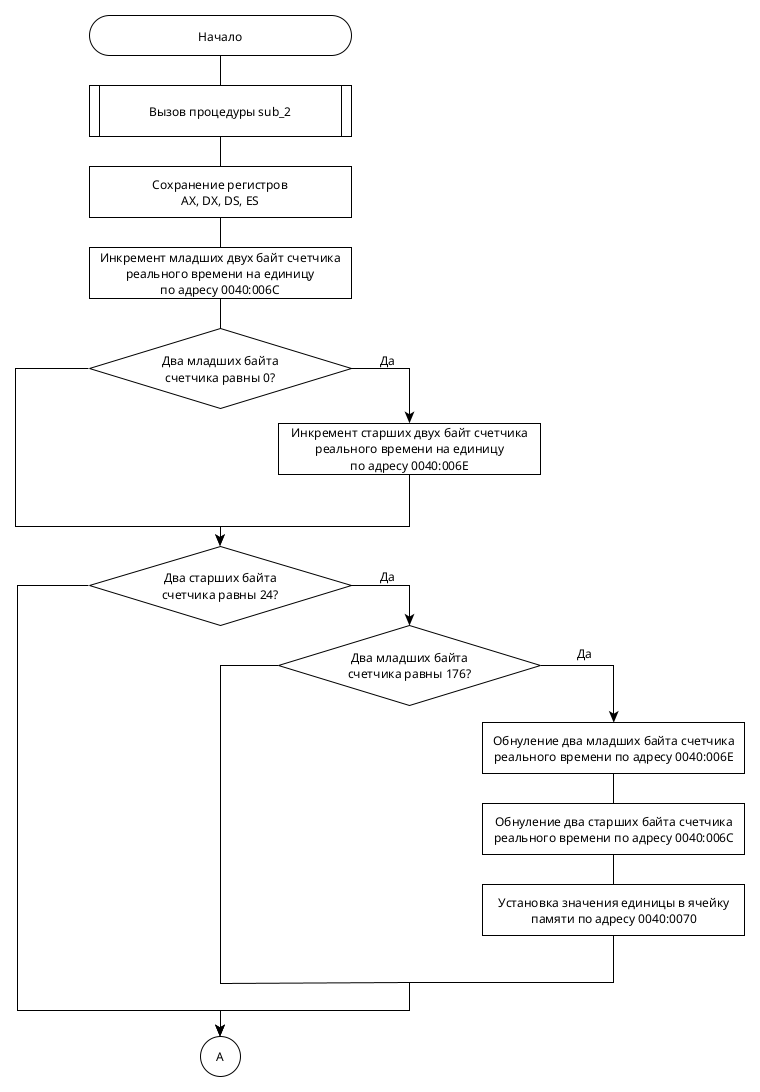
\includegraphics[width=\linewidth]{diagram1_1}
	\end{minipage}

	\pagebreak
	
	\begin{minipage}{0.9\linewidth}
		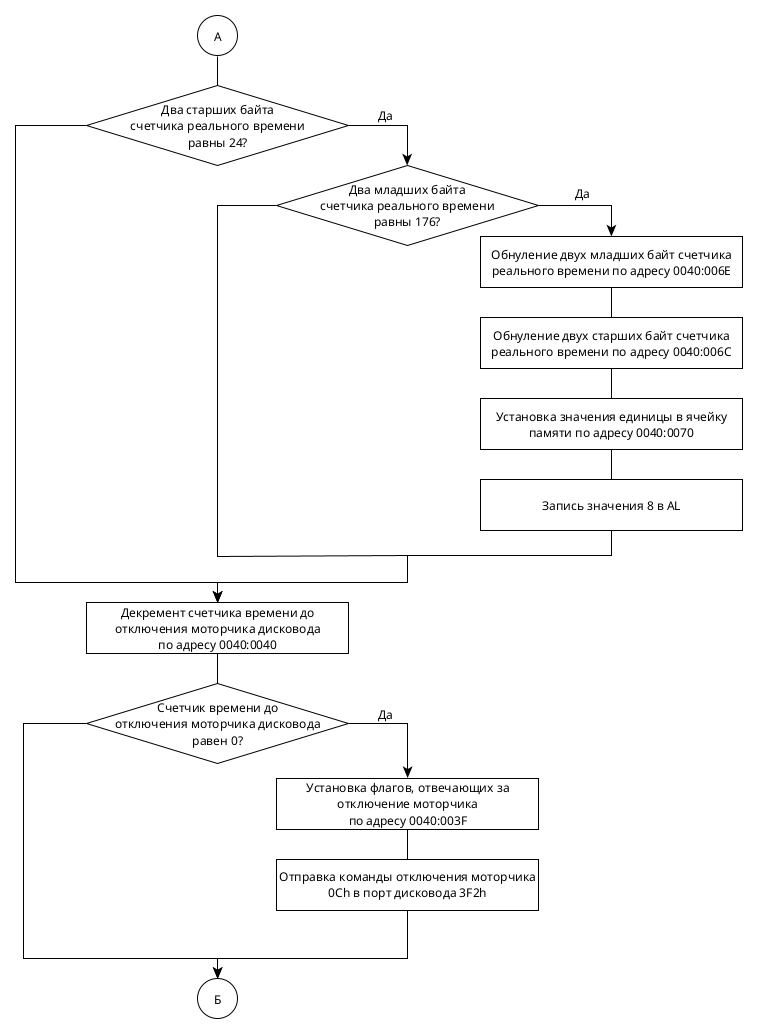
\includegraphics[width=\linewidth]{diagram1_2}
	\end{minipage}

	\pagebreak
	
	\begin{minipage}{0.9\linewidth}
		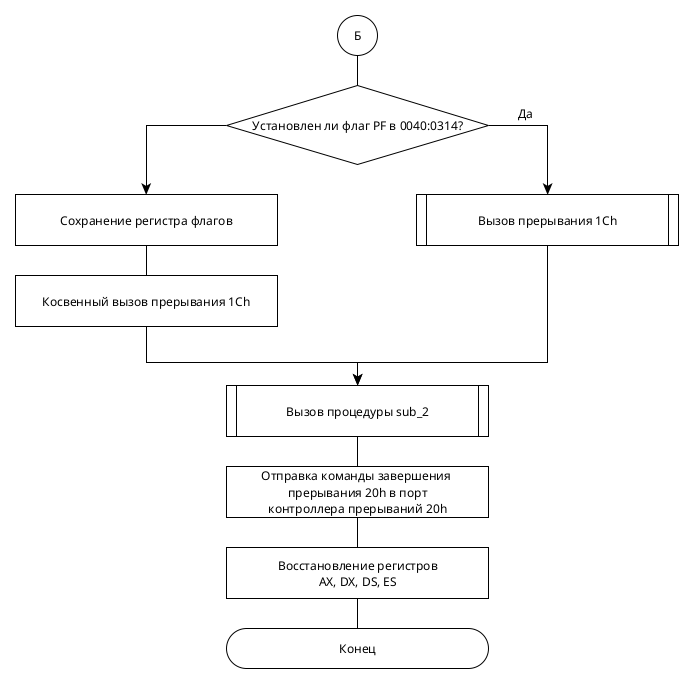
\includegraphics[width=\linewidth]{diagram1_3}
	\end{minipage}

	\pagebreak
	
	\subsection*{Схема алгоритма процедуры sub\_2}
	
	\bigbreak
	
	\begin{minipage}{0.9\linewidth}
		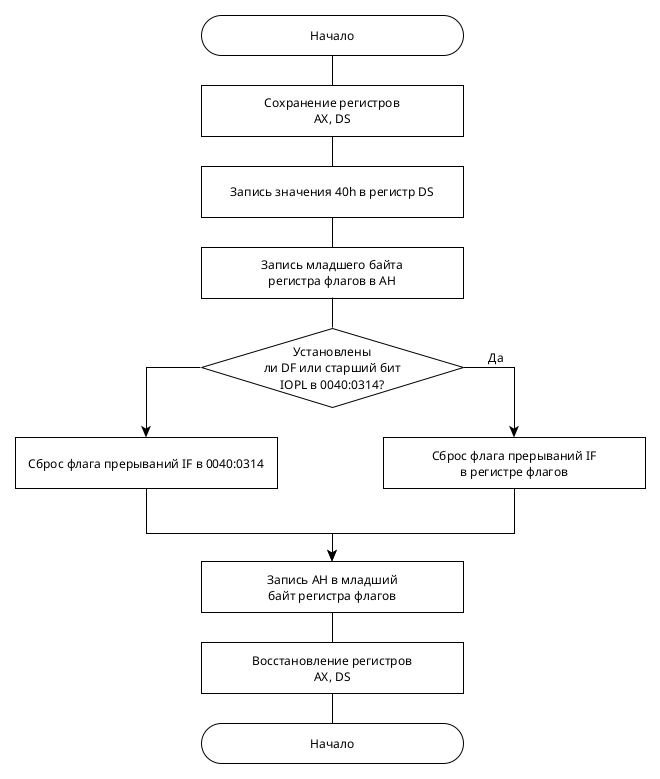
\includegraphics[width=\linewidth]{diagram2}
	\end{minipage}
	
	\pagebreak
	
	\section*{Вывод}
	
	Во время выполнения данной лабораторной работы я познакомился со средством дизассемблирования – sourcer и с получением дизассемблерного кода ядра операционной системы Windows на примере обработчика прерывания Int 8h в virtual mode – специальном режиме защищенного режима, который эмулирует реальный режим работы вычислительной системы на базе процессоров Intel.
	
	Функции обработчика прерывания INT 8h:
	
	\begin{itemize}
		\item Инкремент счетчика реального времени. Обработчик каждый раз увеличивает на единицу текущее значение 4-байтовой переменной, располагающейся в области данных BIOS по адресу 0040:006Ch - счетчик таймера. Если этот счетчик переполнится из-за того что прошло более 24 часов с момента запуска таймера, в ячейку 0000:0470h заносится значение 1.
		
		\item Декремент времени до отключения моторчика дисковода.
		Если после последнего обращения к НГМД прошло более 2 секунд, обработчик прерывания выключает двигатель. Ячейка с адресом 0040:0040h содержит время, оставшееся до выключения двигателя. Это время постоянно уменьшается обработчиком прерывания таймера. Когда оно становится равно 0, двигатель НГМД отключается.
		
		\item Вызов пользовательского прерывания 1Ch.
		Его стандартный обработчик состоит из одной команды IRET.
		Во время выполнения прерывания 1Ch все аппаратные прерывания запрещены.
	\end{itemize}
	
\end{document}
